\documentclass[aspectratio=169,compress]{beamer}

%%%%%%%%%%%%%%%%%%%%%%%%%%%%%%%%%%%%%%%%%%%%%%%%%%%%%%%%%%%%%
% Meta informations:

\title{暗記}
\subtitle{Einführunsveranstaltung, Fachschaft Japanisch}
\author[G. Billing]{Gregor Billing}
\institute[UzK]{Universität zu Köln}
\date[\today]{\today}

%\newcommand{\dtfontscale}{.85}

%%%%%%%%%%%%%%%%%%%%%%%%%%%%%%%%%%%%%%%%%%%%%%%%%%%%%%%%%%%%%
% Languages
\usepackage[ngerman]{babel}

%%%%%%%%%%%%%%%%%%%%%%%%%%%%%%%%%%%%%%%%%%%%%%%%%%%%%%%%%%%%%
% Bind packages:
\usepackage{luatexja}

\usepackage{acronym}						% Acronyms

\usepackage{amsfonts}					% AMS Math Packet (Fonts)
\usepackage{amsmath}						% AMS Math Packet
\usepackage{amssymb}						% Additional mathematical symbols
\usepackage{amsthm}
\usepackage{mathtools}
\usepackage{latexsym}					% Special symbols

\usepackage{booktabs}					% Nicer tables
\usepackage{multicol}					% Content of a table over several columns
\usepackage{multirow}					% Content of a table over several rows

\usepackage{xcolor}						% Enables defining of colors via \definecolor

\usepackage{graphicx}					% Inclusion of graphics
\usepackage[hang]{subfigure}				% Allows to use multiple (partial) figures in a fig

\usepackage{url,xspace,boxedminipage}	% Accurate display of URLs
\usepackage{hyperref}

\usepackage{csquotes}
\usepackage{microtype}

\usepackage{todonotes}
\usepackage{tablefootnote}

%\usepackage[style=authoryear,block=space,backend=biber]{biblatex}
%\addbibresource{src/bib.bib}

%%%%%%%%%%%%%%%%%%%%%%%%%%%%%%%%%%%%%%%%%%%%%%%%%%%%%%%%%%%%%
% Configuration:

\usetheme{Berlin}
\usecolortheme{beaver}

\hyphenation{whe-ther}					% Manually use: "\-" in a word: Staats\-ver\-trag

\DeclareGraphicsExtensions{.pdf,.svg,.jpg,.png,.eps}	% first try pdf, then eps, png and jpg
\graphicspath{{./src/}}								% Path to a folder where all pictures are located

% Tables with a nicer padding:
\renewcommand{\arraystretch}{1.2}
\newcommand{\coordSize}{5.0cm}

%%%%%%%%%%%%%%%%%%%%%%%%%%%%%%%%%%%%%%%%%%%%%%%%%%%%%%%%%%%%%
% Document:
\begin{document}

%\AtBeginSection[]{
%	\begin{frame}[noframenumbering]{Fahrplan}
%		\tableofcontents[currentsection]
%	\end{frame}
%}

%\AtBeginSubsection[]{
%	\begin{frame}[noframenumbering]{Fahrplan}
%		\tableofcontents[currentsubsection]
%	\end{frame}	
%}
%%%%%%%%%%%%%%%%%%%%%%%%%%%
% Content

\begin{frame}
	\titlepage
\end{frame}

\section*{Einführung}

\begin{frame}{Fahrplan}
	\tableofcontents
\end{frame}

\section{Steckbriefe als Faktensammlung}

\begin{frame}{Freunde-Album}
	\begin{columns}[c]
		\column{.5\textwidth}
		\begin{figure}
			
\includegraphics[scale=.15]{horst_steckbrief}
			\caption{Horst}
		\end{figure}
		\column{.5\textwidth} \pause
		\begin{itemize}
			\item \textbf{Wohnort?} \pause Eisenach
			\item \textbf{Beruf?} \pause Tischler
			\item \textbf{Lieblingsfarbe?} \pause Blau
		\end{itemize}
	\end{columns}
\end{frame}

\begin{frame}{Freunde-Album}
	\begin{columns}[c]
		\column{.5\textwidth}
		\begin{figure}
			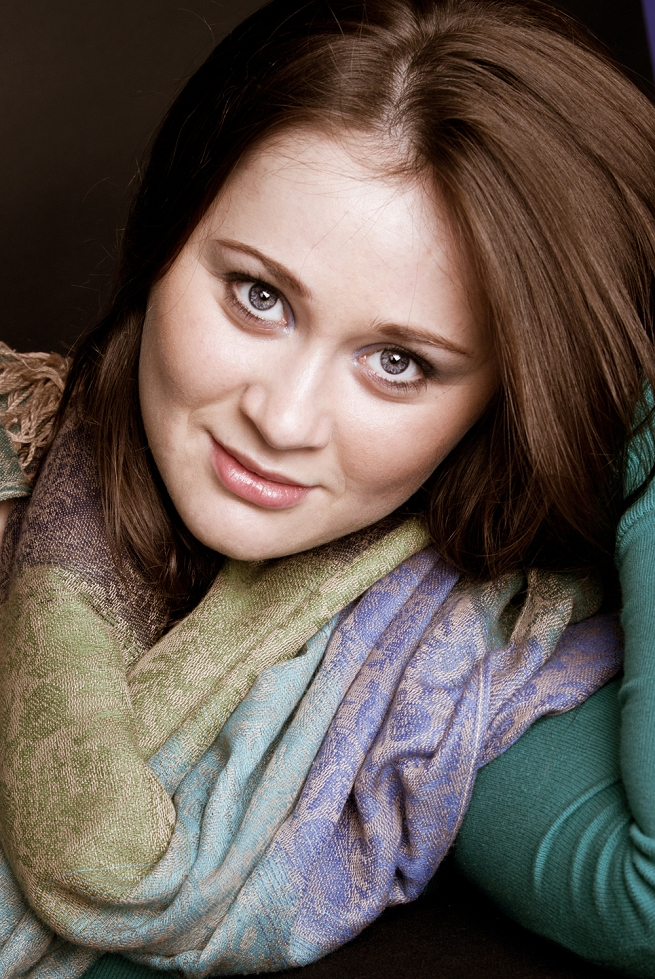
\includegraphics[scale=.135]{brigitte_steckbrief}
			\caption{Brigitte}
		\end{figure}
		\column{.5\textwidth} \pause
		\begin{itemize}
			\item \textbf{Wohnort?} Kiel \pause
			\item \textbf{Beruf?} Bauingenieurin \pause
			\item \textbf{Lieblingsfarbe?} Gelb
		\end{itemize}
	\end{columns}
\end{frame}

\begin{frame}{Freunde-Album}{Dömanenbezug}
	\begin{columns}[c]
		\column{.5\textwidth}
		\begin{figure}
			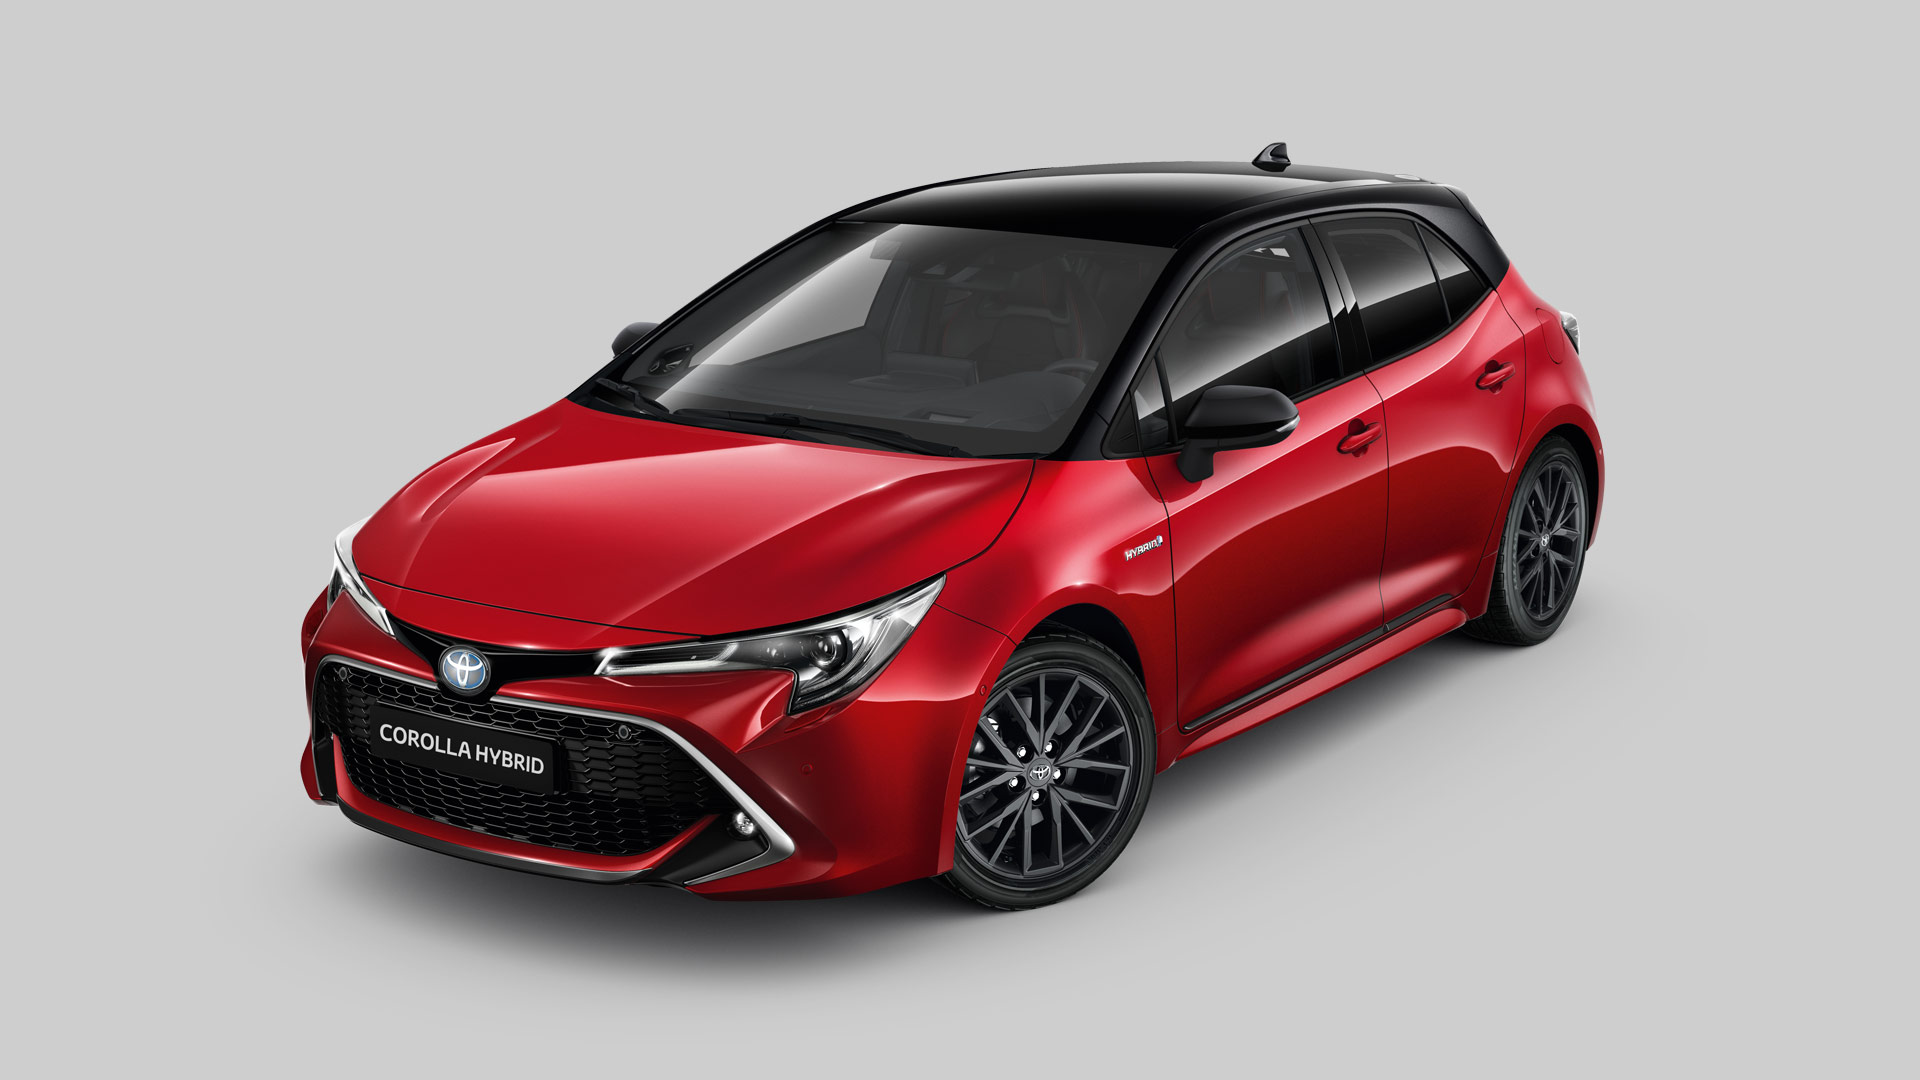
\includegraphics[scale=.085]{toyota_corolla_rot}
			\caption{Toyota Corolla}
		\end{figure}
		\column{.5\textwidth}
		\begin{itemize}
			\item \textbf{Wohnort?} \pause Bauort? \pause Firmensitz? \pause Wohnort des Halters? \pause
			\item \textbf{Beruf?} … \pause
			\item \textbf{Lieblingsfarbe?} ehm?
		\end{itemize}
	\end{columns}
\end{frame}

\begin{frame}{Datenmodell zur Faktenrepräsentation}
	\begin{itemize}
		\item Fakten beziehen sich immer auf spezifische \textbf{Domänen}. Üblicherweise ist das ein Oberbegriff oder eine gemeinsame Gruppe, der die Gegenstände angehören \pause
		\item Abfragen über Fakten sind an ihre Domäne gebunden. Unsere \enquote{Steckbriefe} sind \textbf{domänenspezifisch} \pause
		\item Domänen werden immer durch diejenige Person \textbf{gebunden}, die die Informationen interpretiert. Domänen sind damit \textbf{variabel}
	\end{itemize}
\end{frame}

\begin{frame}{Datenmodell zur Faktenrepräsentation}{Bezug auf Kanji}
	\begin{columns}[c]
		\column{.3\textwidth}
		\center \Huge 漢
		\column{.7\textwidth} \pause
		\begin{itemize}
			\item ON-Lesung
			\item kun-Lesung
			\item Strichzahl
			\item Radikal
			\item (Bedeutung)
		\end{itemize}
	\end{columns}
\end{frame}

\section{Digitales Framework}
\subsection{Installation}

\begin{frame}{Download}
	\begin{itemize}
	\item Frei verfügbare Software auf \url{https://apps.ankiweb.net/}
		\begin{itemize}
			\item Windows
			\item macOS
			\item Linux
		\end{itemize}
	\item Quelloffene Software (das ist gut, da erweiterbar!)
	\item Mobile Clients für Auswendiglernen \enquote{To Go}
		\begin{itemize}
			\item Android
			\item iOS (kostenpflichtig!)
		\end{itemize}
	\end{itemize}
\end{frame}

\subsection{Begriffe}

\begin{frame}{Notizen}{engl. \textit{notes}}
	\begin{itemize}
		\item Notiz-\textbf{Typ}: Anki-Sprech für \textbf{Domänen}
		\item Dargestellt als \textit{key-value-pair}: Frage, Antwort
		\item Identifiziert durch sogenanntes \textbf{Sortierfeld}
		\begin{itemize}
			\item Das beschriebene Faktum muss selbst auch mit in die Notiz aufgenommen werden!
		\end{itemize}
		\item Formatierungsoptionen für bessere Darstellung
		\item Können automatisch mit Schlagworten (\textit{tags}) versehen werden
	\end{itemize}
\end{frame}

\begin{frame}{Karten}{engl. \textit{cards}}
	\begin{itemize}
		\item Unmittelbar an \textit{Notiz-Typen} geknüpft
		\item Spezifiziert Abfrage- und Antwort-Informationen
		\begin{itemize}
			\item \textbf{Vorderseite}: Frage, lerntheoretischer \textit{Input}
			\item \textbf{Rückseite}: Antwort, angestrebter Wissensinhalt
		\end{itemize}
	\end{itemize}
\end{frame}

\begin{frame}{Stapel}{engl. \textit{decks}}
	\begin{itemize}
		\item Sortierstruktur für Notizen und Karten
		\item Hierarchisch angeordnet, Trennsymbol \texttt{::}
		\item Zuordnung eindeutig, man muss sich also für \textit{genau einen} Stapel entscheiden
	\end{itemize}
\end{frame}

\begin{frame}{Stapel}{Strukturhierarchie}
	\begin{columns}[c]
	\column{.5\textwidth}
	\begin{itemize}
		\item Kanji-Workbook
		\begin{itemize}
			\item Band 1
			\begin{itemize}
				\item Kanji
				\item Vokabeln
			\end{itemize}
			\item Band 2
			\begin{itemize}
				\item Kanji
				\item Vokabeln
			\end{itemize}
			\item …
		\end{itemize}
		\item Lehrbuch
		\begin{itemize}
			\item Band 1 (Beginners Vol. 1)
			\begin{itemize}
				\item Vokabeln
				\item Grammatik
			\end{itemize}
		\end{itemize}
	\end{itemize}
	\pause \column{.5\textwidth}
	\begin{itemize}
		\item Kanji-Workbook
		\begin{itemize}
			\item Kanji-Workbook::Band 1
			\begin{itemize}
				\item Kanji-Workbook::Band 1::Kanji
				\item Kanji-Workbook::Band 1::Vokabeln
			\end{itemize}
			\item Kanji-Workbook::Band 2
			\begin{itemize}
				\item Kanji-Workbook::Band 2::Kanji
				\item Kanji-Workbook::Band 2::Vokabeln
			\end{itemize}
			\item …
		\end{itemize}
		\item Lehrbuch
		\begin{itemize}
			\item Lehrbuch::Band 1 (Beginners Vol. 1)
			\begin{itemize}
				\item Lehrbuch::Band 1 (Beginners Vol. 1)::Vokabeln
				\item Lehrbuch::Band 1 (Beginners Vol. 1)::Grammatik
			\end{itemize}
		\end{itemize}
	\end{itemize}
	\end{columns}
\end{frame}

\section{Praktisches Beispiel}
\subsection{Dateneingabe}

\begin{frame}{Notizen \& Karten anlegen}
	\begin{enumerate}
		\item Relevante Informationen festlegen ($\rightarrow$ Notiz-Typ) \pause
		\item Kanji gemäß Notiz-Typ erfassen: 暗、記 \pause
		\item Karten erstellen ($\rightarrow$ HTML-Markup)
	\end{enumerate}
\end{frame}

\subsection{HTML}

\begin{frame}{Intermezzo: HTML-Layout}
	\begin{itemize}
		\item HTML als \textbf{Markup-Sprache}, also Text mit eingebauten Strukturinformationen
		\item Einerseits \textit{Inhalt}, andererseits \textit{Darstellung} dieses Inhalts \pause
		\item Drei wesentliche Funktionsmerkmale
		\begin{enumerate}
			\item \textbf{Was} steht da?
			\item Wo \textbf{fängt} die Strukturinformation \textbf{an}?
			\item Wo \textbf{hört} die Strukturinformation \textbf{auf}?
		\end{enumerate}
	\end{itemize}
\end{frame}

\begin{frame}{Beispiel-HTML}
	Das ist ein Beispiel mit \textbf{fett gedrucktem} Text \par \pause
	\texttt{Das ist ein Beispiel mit <b>fett gedrucktem</b> Text} \pause
	\begin{itemize}
		\item \textbf{Tags}: Strukturinformationen in spitzen \texttt{<Klammern>}
		\item Tag \textbf{schließen}: Forward-Slash
		\item Tags können beliebig tief verschachtelt werden
	\end{itemize}
\end{frame}

\begin{frame}{Notizen \& Karten anlegen}{HTML-Editor}
	Vorder- und Rückseiten einer Karte können beliebiges HTML enthalten. Besonderheiten:
	\begin{itemize}
		\item Inhalte werden dynamisch gefüllt durch \textbf{Templates} auf Grundlage eurer \textit{Notiz-Typen}: \texttt{\{\{Variable\}\}}
		\item Templates können als \textbf{Hint} markiert werden, um nur bei Bedarf eingeblendet zu werden: \texttt{\{\{hint:Radikal\}\}}
		\item Templates können als Teil eines \textbf{Lückentextes} (engl. \textit{cloze}) genutzt werden: \texttt{\{\{cl:Beispielwort\}\}}
		\item Besonderes, reserviertes Template: \texttt{\{\{FrontSide\}\}} für exakte Wiedergabe der Vorderseite auf der Rückseite
	\end{itemize}
\end{frame}

\subsection{Lernen}

\begin{frame}{Abfrage}
	\begin{itemize}
		\item Auswahl eines Stapels startet Lernsequenz
		\begin{itemize}
			\item Pensum üblicherweise voreingestellt
			\item Kann euren persönlichen Präferenzen angepasst werden
		\end{itemize}
		\item Stapel können nach Schlagworten gefiltert werden
		\begin{itemize}
			\item Filtern erstellt temporär neuen Stapel
			\item Jede gelernte Karte wird aus dem Stapel entfernt und in ursprünglichen Stapel zurückgelegt
		\end{itemize}
	\end{itemize}
\end{frame}

\begin{frame}{SRS-Algorithmus}
	\begin{itemize}
		\item Vier Auswahlmöglichkeiten je Abfrage:
		\begin{itemize}
			\item Keine Ahnung
			\item Schwierig
			\item Normal
			\item Einfach 
		\end{itemize}
		\item Je nach gewählter Antwort dauert es länger, bis die Karte erneut abgefragt wird
		\item Erfolgsrezept beruht auf \textbf{Regelmäßigkeit}!!!
	\end{itemize}
\end{frame}

\subsection{Synchronisation}

\begin{frame}{Automatischer Upload}{Cloud von AnkiWeb}
	\begin{itemize}
		\item Die Projektwebsite bietet einen kostenlosen Cloud-Speicher
		\item Synchronisation des Lernfortschritts zwischen Geräten
		\begin{itemize}
			\item Vor dem Start: Prüfen auf neue Informationen
			\item Nach dem Beenden: Hochladen der eigenen Änderungen
		\end{itemize}
		\item \textbf{Synchronisierungskonflikte}: Der Cloud-Server hat Änderungen, mit denen ich nichts anfangen kann (bspw. geänderter Notiz-Typ)
		\item \textbf{ACHTUNG}: Mobile Versionen synchronisieren standardmäßig nicht automatisch!
	\end{itemize}
\end{frame}

\section{Plug-ins}

\begin{frame}{Furigana}
	Plugin: \textit{Japanese Support}, Code: \texttt{3918629684}
	\begin{itemize}
		\item Support für Furigana in eckigen \texttt{[Klammern]}
		\item Mehrere neue Template-Variablen, zum Beispiel:
		\begin{itemize}
			\item \texttt{\{\{furigana:Beispielwort\}\}}
			\item \texttt{\{\{kanji:Beispielwort\}\}}
		\end{itemize}
		\item Weitere Features für Japanisch, wie bspw. eine Lernstandserhebung der Jouyou-Kanji
	\end{itemize}
\end{frame}

\begin{frame}{Strichreihenfolge}
	Plugin: \textit{Kanji Colorizer}, Code: \texttt{1964372878}
	\begin{itemize}
		\item Generiert automatisch farbige Diagramme der Strichreihenfolgen aus dem \textit{KanjiVG}-Projekt
		\item Erkennt Kanji-Felder daran, dass der Notiz-Typ \textit{Japanese} im Namen hat und ein Feld namens \textit{Kanji} sowie \textit{Diagram} existiert
		\item Generierung dauert bei vielen Zeichen mitunter etwas länger…
	\end{itemize}
\end{frame}

\section{Schlusslicht}

\begin{frame}{Vor- und Nachteile}
	\begin{columns}
		\column{.5\textwidth}
		\begin{itemize}
			\item Wiederholung auch alter Karten
			\item Automatische Lernstandserhebung
			\item Wissenskatalog über die Zeit
		\end{itemize}
		\column{.5\textwidth}
		\begin{itemize}
			\item Fehlende Haptik (nur \textit{Recall})
			\item Unter Umständen \textit{zu} strukturiert?!
			\item Ablenkung auf dem Handy (Benachrichtigungen)
		\end{itemize}
	\end{columns} \par \pause
	Anki hilft euch bei der Aufbereitung und Präsentation des Inhalts. Lernen müsst ihr selbst! :)
\end{frame}

\end{document}
